\chapter{Conception}
%Um am Ende der Entwicklung sichergehen zu können, dass das Programm die gewünschte Funktionalität bietet, ist es wichtig zu Beginn die Anforderungen zu definieren und das Projekt nach Abschluss damit zu evaluieren. 
%\section{Anforderungsanalyse}
%%TODO Koen: Wenn dir noch was einfällt, bitte ergänzen (und zwar direkt in den Text)
%Der Fokus dieses Projektes liegt auf die Darstellung und anschauliche Demonstration des Davis Putman Algorithmus anhand des N Damen Problems. Um dieses bestmöglich zu ermöglichen, müssen folgende Anforderungen erfüllt werden. 
%\begin{itemize}
%\item Die Größe von N für das N Damen Problem muss über eine Benutzeroberfläche veränderbar sein
%\item Bei jedem Versuch ein bestimmtes N Damen Problem zu lösen, sollen unterschiedliche Rechenwege und somit auch Lösungen entstehen. Jedoch muss aber gewährleistet sein, dass es jederzeit die Möglichkeit gibt, Ergebnisse replizierbar wiederzuzeigen. 
%\item Der Prozess zur Lösung des N Damen Problems muss einerseits auf einem Schachbrett visuell in einzelnen Schritten gezeigt und andererseits als einzelne Kalkulationsschritte wiedergegeben werden. Dabei muss zur Wahl stehen, ob der Nutzer Macro oder Micro Schritte betrachten möchte. Je nachdem welcher Schritt ausgewählt wurde, ändert sich die Größe der Zwischenschritte.
%\item Die Simualtion muss pausierbar sein.
%\end{itemize}
%Am Ende der Implementierungsphase wird das Programm anhand dieser Anforderungen gemessen und je nachdem als Erfolg oder eben als Nichterfolg deklariert. 

In order to ensure that the program offers the desired functionality at the end of the development process, it is crucial to define the requirements at the beginning and evaluate the project after completion. 
\section{Requirement Analysis}
%TODO Koen: Wenn dir noch was einfällt, bitte ergänzen (und zwar direkt in den Text)
The focus of this project is in the demonstration of the Davis Putman algorithm using the N Queens Problem. In order to achieve this in the best possible way, the following requirements must be met. 
\begin{itemize}
\item The size of N for the N Queens problem has to be modifiable via a user interface
\item With every attempt to solve a certain N Queen problem, different calculation ways and thus also solutions are to develop. However, it must be guaranteed that there is always the possibility to show replicable results. 
\item The process to solve the N Queens problem must be shown visually on a chessboard in individual steps on the one hand and reproduced as individual calculation steps on the other hand. The user must be able to choose between Macro or Micro steps. Depending on which mode was selected, the size of the intermediate steps changes.
\item The simulation must be pausable.
\end{itemize}
At the end of the implementation phase, the program is measured against these requirements and declared as successful or unsuccessful, as the case may be. 

\section{Architecture Sketch}

\section{Layout Design}
Damit die Nutzer die Animation des Davis Putman Algorithmus bestmöglich betrachten können und diesen leicht verstehen können, ist es wichtig, ein anschauliches und übersichtliches Benutzer Interface bereitzustellen. Die Interaktionen und Einstellungsmöglichkeiten müssen selbsterklärend und verständlich sein. Bereits im Vorfeld wurden deshalb verschiedene Ideen zur einem möglichen Layout gesammelt und folgendes Design wurde daraus konzepiert. 
\begin{figure}[h]
  \centering
  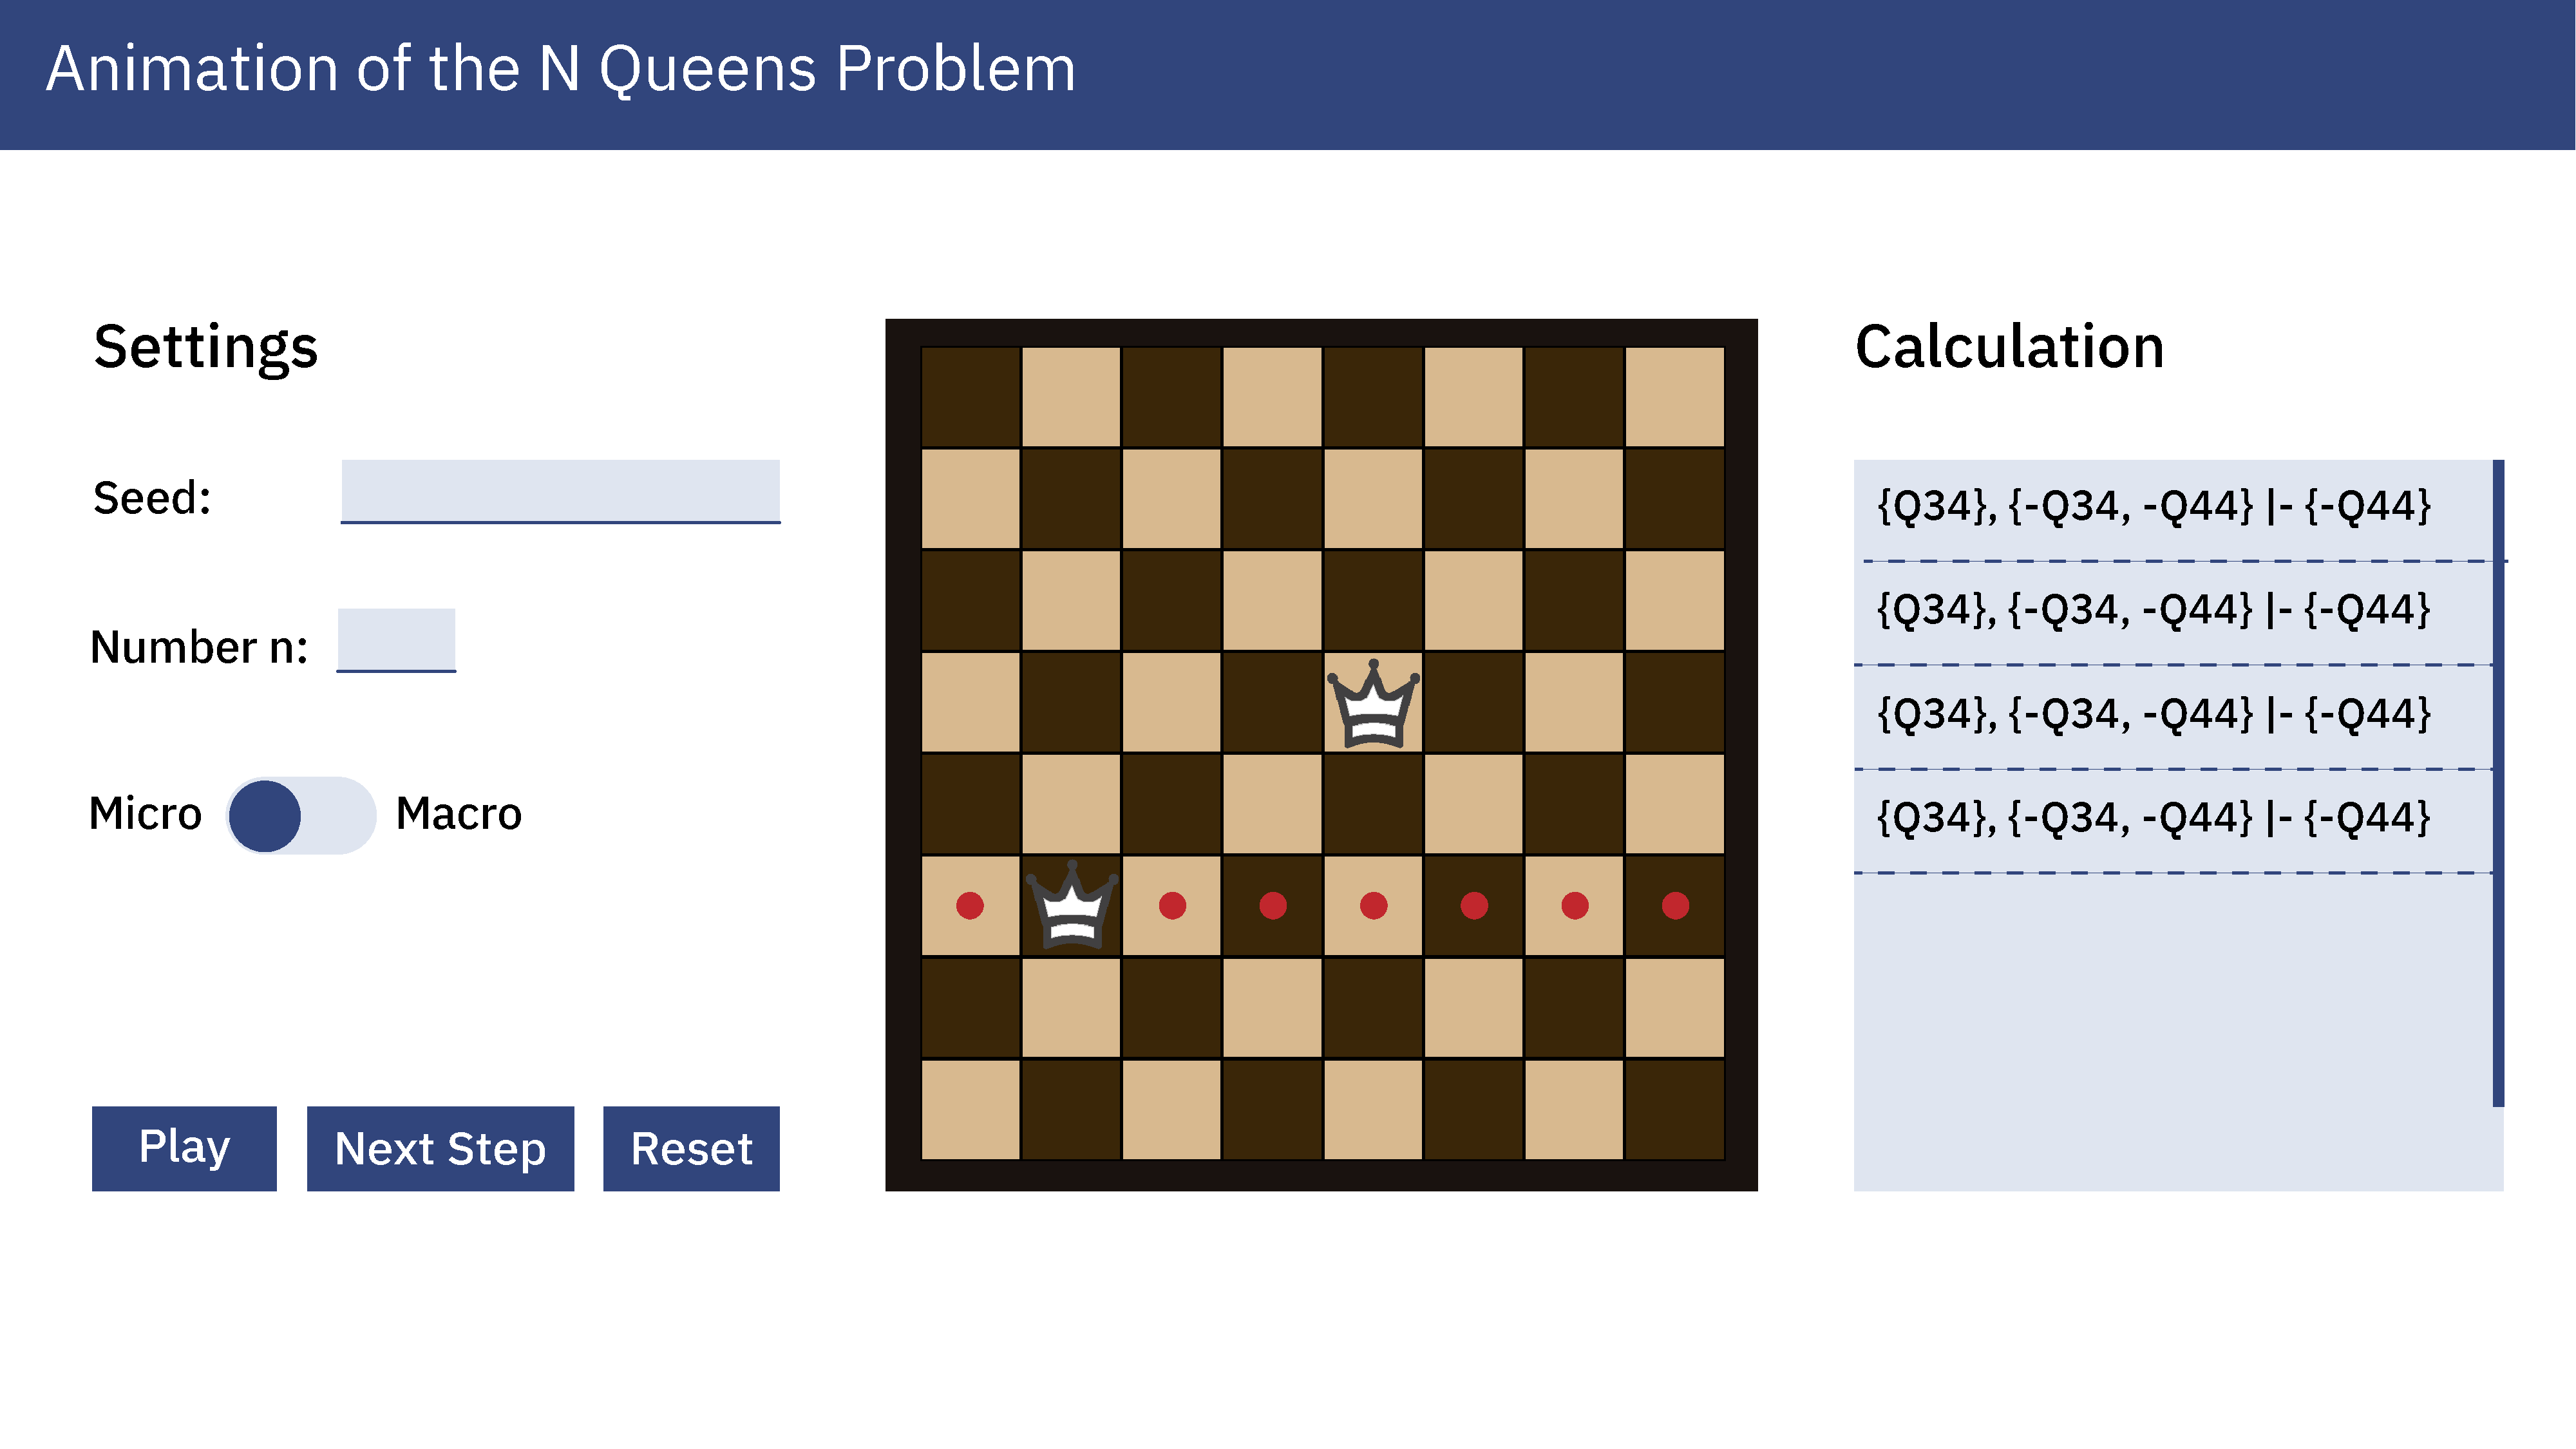
\includegraphics[width=\textwidth]{img/Design_N_Queens}
  \caption{Final Design Sketch for User Interface}
  \label{fig:design}
\end{figure}
Der Header dabei dient als Blickfang, so dass sofort das Thema der Website klar und verständlich heraussticht. Dabei nimmt er die Funktion einer Überschrift ein. 
\\
Darunter wird die Benutzeroberfläche visuell in drei Teile eingeteilt. Dabei befindet sich in der Mitte das Schachbrett, da hier die Hauptanimation stattfindet und somit der Mittelpunkt bilden sollte. Es fängt sofort den Blick der Nutzer ein und leitet sie auf das Hauptgeschehen weiter. 
\\
Links davon befinden sich die Einstellungen zur Animation und Durchführung des Algorithmus. Es entsteht ein natürlicher Lesefluss von links nach rechts, der von den Einstellungen über das Schachbrett hin zu den Kalkulationen geht. Der Nutzer wird inutitiv und selbsterklärend durch das System navigiert, ganz ohne auffällige Steuerungselemente. Die Einstellungen beinhalten dabei nur die wichtigsten Elemente, mit denen die Animation eingestellt werden kann. Dadurch wirkt es nirgends überladen, sondern übersichtlich und strukturiert. Darunter befinden sich die Buttons zur Steuerung der Animation. Je nach Situation wird die Funktionalität dieser angepasst. In diesem Entwurf nehmen die Einstellungen einen festen Platz auf der Oberfläche ein, es gab jedoch durchaus auch die Idee, die Settings in ein aufklappbares sidemenu umzusetzen. Dagegen sprach jedoch die Tatsache, dass der Nutzer dauerhaft mit den Steuerbuttons interagieren muss und aufklappbare Menüs sich nur für einmalige Interaktionen wie beispielsweise die Navigation durch eine Seite anbietet. 
\\
Auf der rechten Seite der Benutzeroberfläche befindet sich die Kalkulation, die den mathematischen Hintergrundprozess in einzelnen Schritten aufzeigt. Die einzelnen Schritte werden dabei in einer scrollbaren Box angezeigt. Ob das oberste Element immer oben bleibt oder die neueren darüber gelegt werden, ist im Design selbst nicht festgelegt.
\\
Wichtig ist, dass alle Komponenten schlüssig miteinander sind. Das bedeutet, dass die Positionierung, der Abstand und das Alignment konsistent sind. Nur dann entsteht am Ende ein stimmiges Gesamtbild. Auch die Farben wurden so gewählt, dass sie beruhigend und in einem einheitlichen Ton, aber mit unterschiedlichen Sättigungen erscheinen. Damit wirkt die Oberfläche harmonisch und nicht überladen. Das Braun des Schachbretts passt sehr gut zum Blauton in der Umgebung und sticht als einzig anderer Farbton aus der Masse hervor. Dieses Farbschema galt jedoch nur zu Demonstrationszwecken und Orientierung. Es kann im Laufe der Implementierung angepasst werden und durch ein passenderes Set ersetzt werden. Ein gut strukturiertes und übersichtliches Layout ist entstanden, welches für die Nutzer leicht verständlich und einfach zu benutzen ist.